\documentclass[12pt,fleqn]{article}\usepackage{../../common}
\begin{document}
Temel Fizik 4 - Atalet Matrisi (Inertia Matrix, Tensor)

Bir objenin havaya fırlatıldığını düşünelim, fırlatma sırasında dönüş te var,
çetrefil bir hareket sözkonusu yani. Fakat şimdiye kadar gördüğümüz teknikler
ile hala bu hareketi analiz edebiliriz, hem lineer momentum, hem de açısal
momentum kütle merkezi odaklı olarak analiz edilebiliyor. Herhangi bir katı
gövde, cisim şeklini ve hareketi analiz için şimdi bazı genel formülleri
ortaya koyalım. 

Gövdenin açısal momentumu $L$ için [1, sf. 379],

$$
L = \sum m_i r_i \times v_i
$$

ki $L,r,v$ vektör. $v = \omega \times r$ eşitliğini üste sokarsak,

$$
L = \sum m_i r_i \times (\omega \times r_i)
\mlabel{1}
$$

Şimdi bu son ifadenin her vektörü öğelerini kullanarak açılımını yapalım böylece
başka bir forma erişmeyi umuyoruz. $\omega = [\begin{array}{ccc} \omega_x&\omega_y&\omega_z \end{array}]^T$
ve $r = [\begin{array}{ccc} x&y&z \end{array}]^T$ öğelerini kullanacağız, ve
üstteki formülün $A \times (B \times C)$ formunda olduğunu farkediyoruz, o zaman
genel bir $r \times (\omega \times r)$ üzerinde BAC-CAB açılımı yapmayı
deneyebiliriz, bu açılım hatırlarsak,

$$
A \times (B \times C) = B(A \cdot C) - C(A \cdot B)
$$

idi. Kendi denklemimiz üzerinde bu açılım

$$
r \times (\omega \times r) = \omega (r \cdot r) - r(r \cdot \omega)
$$

şeklinde olacaktır. Açılımı yapınca 3 x 1 boyutunda bir vektör elde ediyoruz
onun sadece ilk öğesine, $x$ için olan durumuna bakalım,

$$
r \times (\omega \times r)_x = \omega_x (x^2 + y^2 + z^2) - x(\omega_x x + \omega_y y + \omega_z z)
$$

$\omega_x x^2$ iki yerden iptal olur, kalanlar,

$$
 = \omega_x ( y^2 + z^2) - \omega_y xy + \omega_z xz
$$

Her üç öğe için açılım yapınca,

$$
r \times (\omega \times r) =
\left[\begin{array}{c}
(y^2 + z^2) \omega_x - xy \omega_y - xz \omega_z \\
-yx \omega_x + (z^2 + x^2)\omega_y - yz \omega_z \\    
-zx \omega_x - zy \omega_y + (x^2+y^2)\omega_z
\end{array}\right]
$$

Ve ana formülde $m_i$ çarpımı olduğunu unutmayalım,

$$
m r \times (\omega \times r) =
\left[\begin{array}{c}
m (y^2 + z^2) \omega_x - m xy \omega_y - m xz \omega_z \\
-m yx \omega_x + m (z^2 + x^2)\omega_y - m yz \omega_z \\    
-m zx \omega_x - m zy \omega_y + m (x^2+y^2)\omega_z
\end{array}\right]
$$

Ustteki sonucu (1)'e sokunca, ve notasyonel olarak bazı rahatlıklar düşünerek,
mesela $I_{xx} = \sum_i m_i (y_i^2 + z_i^2)$ gibi, ya da $I_{xy} = - \sum_i m x_i y_i$.
Bunları da yerine koyunca, $L_x,L_y,L_y$ diyelim,

$$
L_x = I_{xx} \omega_x + I_{xy} \omega_y + I_{xz} \omega_z
$$

$$
L_y = I_{yx} \omega_x + I_{yy} \omega_y + I_{yz} \omega_z
$$

$$
L_z = I_{zx} \omega_x + I_{zy} \omega_y + I_{zz} \omega_z
$$

Fakat bu son sonuç hala biraz sadeleştirilebilir. İfadeye bakarsak onu bir
matris çarpı bir vektör çarpımı ile temsil edebiliriz gibi geliyor,
hakikaten de

$$
I = \left[\begin{array}{ccc}
I_{xx} & I_{xy} & I_{xz} \\
I_{yx} & I_{yy} & I_{yz} \\
I_{zx} & I_{zy} & I_{zz} 
\end{array}\right], \quad
\omega = \left[\begin{array}{c}
\omega_x \\ \omega_y \\ \omega_z
\end{array}\right]
$$

üzerinden $I \omega$ çarpımının (2) sonucunu vereceğini görebiliriz. Böylece
gayet sade

$$
L = I \omega
$$

ifadesine geri gelmiş olduk.

$I$, atalet matrisidir, ve her katı kütle şekline göre farklı olacak bir
matristir. O zaman bir objenin açısal momentumunun nasıl olacağını hesaplamak
için önce o objenin atalet matrisine hesaplamak gerekir.

Ataletin Ana Eksenleri (Principal Axes of Inertia) 

Bir konu daha var tabii; dikkat edersek $I$ matrisini çekip çıkardığımız hesap
bir $O$ referansını merkez alıyordu. ``Genel bir $O$ olsun'' dedik ve oradan
türetmeye devam ettik. Fakat bazı referansların, yani dönüşün neyin etrafında
olduğunun, her seçime göre farklı $I$'lara sebebiyet verebileceğini görmek
gerekir. Lineer cebirsel olarak $L$ ile $\omega$'nin aynı yönü göstermesi için
$I$'nin köşegen matris olması gerekir. Fakat elde köşegen matris olmasa da
$\omega$'yi bizim değiştirerek, aynı refarans $O$'dan geçen ama farklı öyle bir
yönü göstermektir ki, bu eksen etrafında bir köşegen $I$ elde edilsin ve hareket
simetrik hale gelsin.

Bu hesap için özdeğer, özvektör hesabını yapmak lazım, ya da atalet matrisinin
köşegenleştirilmesini [2] (diagonalization) gerçekleştirmek lazım. Eğer $I$
köşegen değil ise, öyle bir $\omega$ bulalım ki $L = I \omega$ hesabındaki
$L$, $I \omega$ ile aynı yönü göstersin, yani

$$
I\omega = \lambda \omega
$$

haline gelsin. Bu bir özdeğer problemi değil midir? Evet. 

Örnek olarak [1, sf. 382]'deki $O$ etrafında dönen küp orneğini kullanalım,

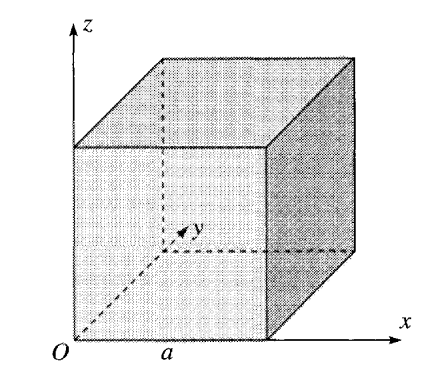
\includegraphics[width=20em]{phy_005_basics_04_01.png}

Bu referansa göre atalet matrisi

$$
I = \left[\begin{array}{rrr}
8 & -3 & -3 \\
-3 & 8 & -3 \\
-3 & -3 & 8
\end{array}\right]
$$

olarak bulunmuş. Görüldüğü gibi $I$ köşegen değil. Kosegenlestirmek icin,

\begin{minted}[fontsize=\footnotesize]{python}
import numpy.linalg as lin
I = np.array([[8, -3, -3],
              [-3, 8, -3],
              [-3, -3, 8]])
e,evec = lin.eig(I)
print (e)
print (evec)
print (evec[:,0])
\end{minted}

\begin{verbatim}
[11.  2. 11.]
[[ 0.81649658 -0.57735027  0.        ]
 [-0.40824829 -0.57735027 -0.70710678]
 [-0.40824829 -0.57735027  0.70710678]]
[ 0.81649658 -0.40824829 -0.40824829]
\end{verbatim}

Demek ki yeni $I$ matrisi

$$
I = \left[\begin{array}{rrr}
11 & 0 & 0 \\
0 & 2 & 0 \\
0 & 0 & 11 
\end{array}\right]
$$

olmalı.

Üç tane $\omega$ vektörü elde edildi, bunlar tabii ki birbirine dik, hepsini
grafikleyelim, yeşil çizgiler $x,y,z$ eksenleri olmak üzere,

\begin{minted}[fontsize=\footnotesize]{python}
from mpl_toolkits import mplot3d

def plot_vector(fig, orig, v, color='blue'):
   ax = fig.gca(projection='3d')
   orig = np.array(orig); v=np.array(v)
   ax.quiver(orig[0], orig[1], orig[2], v[0], v[1], v[2],color=color)
   ax = fig.gca(projection='3d')  
   return fig

fig = plt.figure()
axes = mplot3d.Axes3D(fig)
SCALE = 0.5
plot_vector(fig, [0,0,0],evec [:,0]*SCALE)
plot_vector(fig, [0,0,0],evec [:,1]*SCALE)
plot_vector(fig, [0,0,0],evec [:,2]*SCALE)
axes.view_init(elev=10, azim=200)
axes.set_xlim(-1,1)
axes.set_ylim(-1,1)
axes.set_zlim(-1,1)
axes.plot([0,1],[0,0],[0,0],color = 'g')
axes.plot([0,0],[0,1],[0,0],color = 'g')
axes.plot([0,0],[0,0],[0,1],color = 'g')
axes.locator_params(tight=True, nbins=4)
plt.savefig('phy_005_basics_04_02.png')
\end{minted}

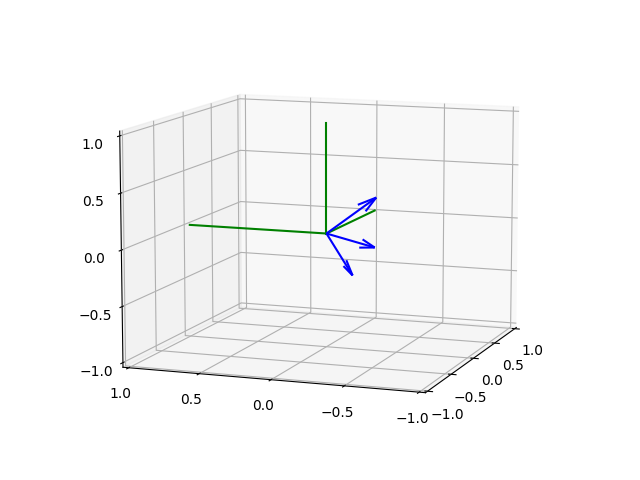
\includegraphics[width=20em]{phy_005_basics_04_02.png}

Rotasyon Matrisi ve Türevi

Bir 3 x 3 dönüş matrisi ile herhangi bir vektörü döndürebileceğimizi biliyoruz.
Yersel taşıma daha da basit, 3 boyutlu bir vektör sadece, mevcut konuma
ekleyerek yeni konumu elde ediyoruz.

Bir katı gövdeyi parçacıkları üzerinden alırsak, ve bu gövdenin açısal dönüşsel
olarak hangi yöne baktığını bir dönüş matrisi $R$ ile temsil edersek, her
parçacık üzerinde bu işlemin uygulandığını düşünebiliriz. Ayrıca konumsal
taşınma ve bakılan yön başlangıçtaki bir ``gövde uzayı''na (body space) göre
yapılabilir, gövdenin kütle merkezini dünya kordinatlarının (0,0,0) orijin
noktasında ve yönü herhangi bir (başta belli) yöne doğru alalım, hareketler hep
bu konuma referansla, onu değiştirecek şekilde düşünülebilir.  Mesela gövde
üzerindeki, gövde uzayındaki, herhangi bir $p_0$ noktasını düşünelim, $t$ anında
bu noktanın dünya uzayındaki konumu

$$
p(t) = R(t) p_0 + \chi(t)
$$

ki $\chi(t)$ bir yersel taşınma, ve $R(t)$ açısal dönüş. Tabii taşınma her zaman
kütle merkezine uygulandığı için $a(t)$ aynı zamanda kütle merkezinin her $t$
anında dünya uzayında olduğu yeri de gösteriyor.

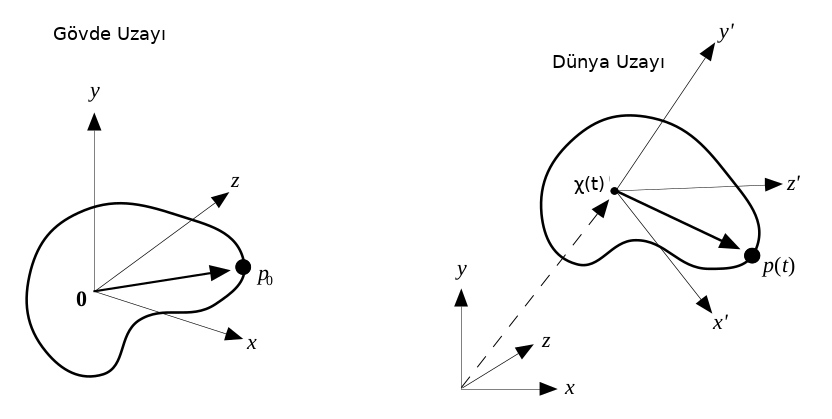
\includegraphics[width=20em]{phy_005_basics_04_04.png}

Türeve gelirsek, bir vektör $r$'nin orijin etrafında döndüğünü
düşünelim. Herhangi bir anda bu dönüşün açısal hızı $\omega$ çapraz çarpımla
hesaplanabilir,

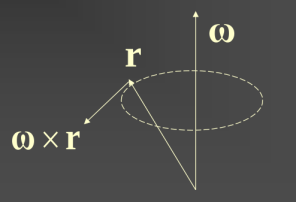
\includegraphics[width=10em]{phy_005_basics_04_03.png}

Hız tabii ki sonsuz küçük zamandaki yer değişimi olduğu için onu

$$
\frac{\ud r}{\ud t} = \omega \times r
$$

olarak ta görebiliriz. Şimdi bir katı gövdeyi düşünelim, onun baktığı yön
(orientation) bir matris $R$ içinde. Bu matrisin her kolonunda bir eksen var,
ilk kolon $x$, ikinci $y$, vs. Eğer gövdenin baktığı yönü $R$ ile temsil
ediyorsak tüm bu kolonlar gövde dönerken değişecektir. Eğer dönüş $\omega$ ise
her eksenin açısal hızı $\omega$ demek, o zaman bu eksenlerin, $b,c,d$ diyelim,
açısal hızı ayrı ayrı $\omega \times b$, $\omega \times c$, $\omega \times d$
olarak bulunabilir, ki bunların her biri aynı zamanda ayrı birer türevdir. Tüm
matrisin türevi

$$
\frac{\ud R}{\ud t} = \tilde \omega \cdot R
$$

ki $\tilde \omega$ ile $\omega$'yi eksi bakışımlı [4] bir matris hale getirdik,
böylece çapraz çarpımı noktasal çarpım haline çevirmiş oluyoruz [5, sf. 9], [3].

Atalet Matrisi ve Dönüşler

Daha önce atalet matrisi $I(t)$'yi görmüştük,

$$
I(t) = \sum \left[\begin{array}{ccc}
m_i (y_i^2 + z_i^2) & -m_i x_i y_i & m_i x_i z_i \\
-m_i y_i x_i & m_i (x_i^2 + z_i^2) & -m_i y_i z_i \\
-m_i z_i x_i & -m_i z_i y_i & m_i (x_i^2 + y_i^2)
\end{array}\right]
$$

Burada $x,y,z$ değerleri gövde uzayında, her nokta $r_i'$ için $x_i,y_i,z_i$
değerleri $r_i - \chi(t)$ içeriğiyle hesaplanıyor. Ayrıca bir obje dönerse, onun
belli noktalarının eksenden olan uzaklıkları değişir ve farklı bir $I$ elde
ederiz... fakat üstteki hesabı obje hareket ederken sürekli yapmak oldukca
külfetlidir. Acaba $I$'nin bir baz kısmını hesaplasak, sonra dönüşe göre onu
güncellesek olmaz mı?

Bunun bir yolu var [5, sf. 14]. $r_i'^T r_i' = x_i^2 + y_i^2 + z_i^2$ olduğundan
hareketle, önceki $I$ denklemini şu şekilde yazabiliriz,

$$
I(t) = \sum
m_i r_i'^T r_i' \left[\begin{array}{ccc}
1 & 0 & 0 \\ 
0 & 1 & 0 \\ 
0 & 0 & 1 
\end{array}\right] -
\left[\begin{array}{ccc}
m_i x_i^2 & -m_i x_i y_i & m_i x_i z_i \\
-m_i y_i x_i & m_i y_i^2 & -m_i y_i z_i \\
-m_i z_i x_i & -m_i z_i y_i & m_i z_i^2
\end{array}\right]
$$

Simdi en sağdaki matrise dikkat edelim, onu bir dış çarpım (outer product)
olarak temsil edebiliriz, alttaki gibi,

$$
r_i' r_i'^T = \left[\begin{array}{c}
x_i \\ y_i \\ z_i
\end{array}\right]
\left[\begin{array}{ccc}
x_i & y_i & z_i
\end{array}\right] =
\left[\begin{array}{ccc}
x_i^2 &  x_i y_i &  x_i z_i \\
y_i x_i & y_i^2 & y_i z_i \\
z_i x_i & z_i y_i & z_i^2
\end{array}\right]
$$

Bunu kullanarak ve 3 x 3 boyutlu birim matrisini $\vec{1}$ ile göstererek
(normalde bu matris için $I$ notasyonu kullanılır ama o hard bu yazıda
kapılmış durumda),

$$
I(t) = \sum m_i ((r_i'^T r_i') \vec{1} - r_i' r_i'^T)
$$

Bu nasıl faydalı? Çünkü $r_i(t) = R(t) r_{0i} + \chi(t)$ ki $r_{0i}$ başlangıçtaki
kütlede $i$ parçacığınin yeri, ve sabit, o zaman

$$
r_i(t) - \chi(t) = R(t) r_{0i} = r_i'(t)
$$

Şimdi $r_i'(t) = R(t) r_{0i}$ eşitliğini iki üstteki formülde kullanırsak,

$$
I(t) = \sum
m_i ( (R(t) r_{0i})^T  (R(t) r_{0i})  \vec{1} -  (R(t) r_{0i})  (R(t) r_{0i})^T  )
$$

$$
= \sum
m_i ( r_{0i}^T R(t)^T R(t) r_{0i} \vec{1} -  R(t) r_{0i} r_{0i}^T R(t)^T )
$$

$R(t)$ dikgen, ortonormal matris oldugu icin $R(t)^TR(t) = \vec{1}$

$$
= \sum
m_i ( (r_{0i}^T r_{0i}) \vec{1} -  R(t) r_{0i} r_{0i}^T R(t)^T )
$$


Üstteki formülde ikinci terimde $R(t) .. R(t)^T$ ifadesi var, bunu
birinci terime de eklemek için, ve $r_{0i}^T r_{0i}$ bir tek sayı değer
olduğu için ve $R(t) R(t)^T$'nin birim matris olmasından hareketle,

$$
= \sum
m_i ( R(t) (r_{0i}^T r_{0i}) R(t)^T \vec{1} -  R(t) r_{0i} r_{0i}^T R(t)^T )
$$

Böylece $R(t)$ ve $R(t)^T$ dışarı çekilebiliyor,

$$
= R(t) \left( \sum 
m_i (( r_{0i}^T r_{0i}) \vec{1} -  r_{0i} r_{0i}^T
\right)  R(t)^T 
$$

Böylece parantez içindeki, $I_{body}$ denebilecek değerler parçacıkların
gövdenin ilk konumundaki yerlerine (ve değişmeyen kütle $m_i$ değerine) göre
hesaplanabileceği için, onu bir kez hesaplayabiliriz, ve sonra ona $R(t)$'leri
uygulayarak istediğimiz güncel $I(t)$ değerini elde ederiz.

$$
I(t) = R(t) I_{body} R(t)^T
$$

Hareketin Kati Govde Denklemleri






[devam edecek]

Kaynaklar

[1] Taylor, {\em Classical Mechanics}

[2] Bayramlı, {\em Lineer Cebir, Ders 22}

[3] Rotenberg, {\em CSE169: Computer Animation, UCSD}

[4] Bayramlı, {\em Lineer Cebir, Ders 5}

[5] Witkin, {\em Physically Based Modeling}

\end{document}




